%!TEX root = ../../../adrien_gomar_phd.tex
\chapter{Fourier-based methods}
\label{cha:spectral_methods}

\chabstract{The four main
Fourier-based methods are presented in this chapter: the Linearized 
Unsteady Reynolds-averaged Navier--Stokes (LUR), 
the Non-Linear Harmonic (NLH), 
the Non-Linear Frequency Domain (NLFD) 
and the Harmonic Balance (HB) methods. The LUR
method comes from a linearization of the governing equations
while the three others are built to take into account for the 
non-linearities. The NLH, NLFD and HB methods
rely on a decomposition of the variable of interest
in Fourier series. By truncating these at order $N$,
$2N+1$ steady equations coupled by
a source term are obtained. 
Emphasis is put on the development
of the multi-frequential formulation and its
mathematical background to allow multi-frequential applications.
This is the case, for instance, of a pylon-rotor-rotor configuration
(namely an installed CROR) or a CROR with a moving blade, which is
the purpose of the current thesis.
The applicability of 
these methods is demonstrated in the literature
through analytical test cases, $2$D/$3$D academic 
turbomachine configurations,
industrial subsonic/transonic multi-stage applications, 
aeroelastic configurations and even unsteady
optimization problems. The cost of the methods
is almost $2N+1$ times the cost of a steady
computation with $N$ being the number of computed harmonics.}

\minitoc
\newpage

% ================
% = INTRODUCTION =
% ================
\section{Introduction}
\label{sec:sm_intro}
%!TEX root = ../../adrien_gomar_phd.tex

The computational power available today in
the research centers and in the industry
is so big that large eddy simulation
becomes possible for some industrial configurations.
This is actually needed as high-fidelity
simulations help the turbomachinery community understand
the complex nature of flows that develop 
within these components,
allowing breakthrough ideas.
However, even if high fidelity approaches
are today within reach, it is still a challenge for
multi-row configurations.
Moreover, they will always be room for fast reliable
computations. 
As a matter of fact, on a daily basis, engineers need
to run lots of simulations to test new designs.
In this framework, large eddy simulation is
too demanding to be used for design purposes.

Today, in most companies, steady Reynolds-Averaged
Navier-Stokes (RANS) based solver are used on a daily basis.
For instance, this tool 
helped building the new $3$D-shape
of the forthcoming CFM-LEAP engine
depicted in Fig.~\ref{fig:sm_leap}.
\begin{figure}[htbp]
  \centering
  \includegraphics*[width=0.40\textwidth]{leap.jpg}
  \caption{$3$D-shape fan blades of the forthcoming CFM-LEAP engine.}
  \label{fig:sm_leap}
\end{figure}
Some further improvements are made possible by the use
of the unsteady RANS computations.
However, in the industry, unsteady computations
are still too expensive to be used on a daily basis.
Based on a simple idea, spectral methods are 
able to reproduce the unsteady field to engineering
accuracy, for a cost proportional to the cost of a
steady computation.

In turbomachines, the relative speed motion between the blades
give rise to inherent time-periodic phenomena.
In fact, consider a stage of a turbomachine, as for instance
a turbine stator-rotor configuration as shown 
in Fig.~\ref{fig:sm_unsteady_turbomachine}. 
\begin{figure}[htbp]
  \centering
  \includegraphics*[width=0.4\textwidth]{unsteady_turbomachine.pdf}
  \caption{Main unsteady effects present in a turbomachinery stage. Here, a turbine stator-rotor
  configuration is shown.}
  \label{fig:sm_unsteady_turbomachine}
\end{figure}
Due to the
viscosity effects acting on the stator blades, 
a wake is generated behind it and 
impinges the rotor row. In opposite, the flow field
generated around the rotor can literally go back up
to the stator row. In fact
the acoustic fluctuations can go backwards yielding
the potential effects. Moreover as, the rows have a 
rotation speed difference,
the field that is created in one row is perceived as unsteady in the opposite 
row frame of reference. This unsteadiness can be
correlated with the so-called Blade Passing Frequency (BPF) defined as:
\begin{equation}
	f = \frac{\Omega_{rel} B_{opp}}{2 \pi},
\end{equation}
where $f$ is the BPF, $\Omega_{rel}$ the relative speed difference 
and $B_{opp}$ the number of blades in the opposite row.
At first order, the unsteady effects presented here drive
most of the time-dependent field in a turbomachine. This 
is of course an approximation, but we will see at the end
of this chapter that the range of unsteady periodic
flow phenomenon in a CROR is large.

The problem with classical time-marching scheme is 
that it has no knowledge
of the periodic nature of the field yielding a time-consuming
transient. Thus, one idea is to build efficient algorithm
by taking advantage of this periodicity. 
Hence the spectral methods that are
presented above.



\section{The \underline{L}inearized 
\underline{U}nsteady \underline{R}eynolds-averaged Navier--Stokes method (LUR)}
\label{sub:sm_lur}
%!TEX root = ../../../adrien_gomar_phd.tex

\citet{Verdon1984} originally developed the unsteady linearized 
method in the framework of potential flows. Later on, \citet{Hall1989}
extended it to the Euler equations and
\citet{Clark2000} applied it to the Reynolds-Averaged Navier--Stokes equations,
yielding the LUR method.
This method relies on a decomposition of the variables
into a base part (generally the steady-state) 
and a small-disturbance unsteady component
\begin{equation}
	u = \overline{u} + u^\prime,
	\label{eq:sm_lur_decomposition}
\end{equation}
where $u^\prime$ is considered to be a small unsteady perturbation.
In his PhD thesis,
\citet{Hall1987} defines small to be less than $10\%$ of the
steady flow.
Injecting Eq.~\eqref{eq:sm_lur_decomposition} into 
Eq.~\eqref{eq:sm_nonlinear_convection_conservative} yields
\begin{equation}
	\frac{\partial u^\prime}{\partial t} + 
	\frac{1}{2}\frac{\partial}{\partial x} \left[
	\overline{u}^2 + 2 \overline{u} u^\prime + u^\prime u^\prime \right] = 
	0.
	\label{eq:sm_lur_step_1}
\end{equation}
By means of linearization, \emph{i.e.} collecting terms
of equal order (equivalently $\overline{u^\prime} = 0$) 
and neglecting terms of order greater than one, 
Eq.~\eqref{eq:sm_lur_step_1} can be split
into a steady equation
\begin{equation}
	\frac{1}{2} \frac{\partial \overline{u}^2}{\partial x} = 0,
	\label{eq:sm_lur_step_2}
\end{equation}
and an unsteady first-order perturbation equation
\begin{equation}
	\frac{\partial u^\prime}{\partial t} +
	\frac{\partial}{\partial x} \left[
	\overline{u} u^\prime \right] = 
	0.
	\label{eq:sm_lur_step_3}
\end{equation}
There is a one-way coupling between the two equations:
the steady field
is first computed using Eq.~\eqref{eq:sm_lur_step_2}
and is secondly given as an input to the
perturbation equation to compute
the corresponding unsteady disturbance (Eq.~\eqref{eq:sm_lur_step_3}). 
However, the computed
perturbation is not used to update the steady solution.
Hence the one-way coupling.

\subsection{Mono-frequential formulation}
As mentioned before, Fourier-based time methods have been developed to efficiently
capture periodic phenomena.
Hence, assuming that the velocity perturbation is harmonic with 
angular frequency $\omega$, one can write
\begin{equation}
	u^\prime = \widehat{u}_1 e^{i \omega t} + \widehat{u}_{-1} e^{-i \omega t},
\end{equation}
with $\widehat{u}_1$ and $\widehat{u}_{-1}$ being complex conjugates giving a
real value for the perturbation.
Injecting this definition into Eq.~\eqref{eq:sm_lur_step_3} and using
the orthogonality property of the complex exponentials leads
to
\begin{equation}
	\begin{dcases}
		i \omega \widehat{u}_1 +
		\frac{\partial}{\partial x} \left[
		\overline{u} \widehat{u}_1 \right] &= 
		0, \\
		-i \omega \widehat{u}_{-1} +
		\frac{\partial}{\partial x} \left[
		\overline{u} \widehat{u}_{-1} \right] &= 
		0.
	\end{dcases}
	\label{eq:sm_lur_step_4}
\end{equation}
Finally a pseudo-time $\tau$ is added to time-march 
Eq.~\eqref{eq:sm_lur_step_2} and Eq.~\eqref{eq:sm_lur_step_4}
to the steady-state, giving three equations in total
\begin{alignat}{2}
	\fbox{$
	\begin{dcases}
		\frac{\partial \overline{u}}{\partial \tau} +
		\frac{\partial 
			\overline{u}^2}{\partial x} &= 0, \\
		\frac{\partial \widehat{u}_1}{\partial \tau} +
		i \omega \widehat{u}_1 +
			\frac{\partial}{\partial x} \left[
			\overline{u} \widehat{u}_1 \right] &= 
			0, \\
		\frac{\partial \widehat{u}_{-1}}{\partial \tau}
		-i \omega \widehat{u}_{-1} +
			\frac{\partial}{\partial x} \left[
			\overline{u} \widehat{u}_{-1} \right] &= 
			0
	\end{dcases}
	$}
\end{alignat}

\subsection{Extension to the Navier--Stokes equations}
To extend the LUR method to the Reynolds-Averaged
Navier--Stokes equations, one has to consider
their linearized counterpart.
The reader is referred to the paper of \citet{Clark2000} for
a detailed development of the LUR method for the Navier--Stokes
equations.

\subsection{Numerical cost}
As the method is based on three equations in total, one steady equation 
(namely a classical RANS equation) and two perturbation equations, 
if $\mathdollar_{\text{RANS}}$ 
denotes the CPU and memory cost of
one steady computation, then the cost of the LUR
method can be estimated as
\begin{equation}
	\mathdollar_{\text{LUR}} = 3 \times \mathdollar_{\text{RANS}}.
\end{equation}
In practice, only two computations are performed since the steady computation
is usually available beforehand.


\section{The \underline{N}on-\underline{L}inear 
\underline{H}armonic method (NLH)}
\label{sub:sm_nlh}
%!TEX root = ../../../adrien_gomar_phd.tex

Originally developed by \citet{He1998} and \citet{Ning1998},
the NLH method
relies on a decomposition of the conservative variables into a
time-averaged part plus an unsteady perturbation
\begin{equation}
	u = \overline{u} + u^\prime,
	\label{eq:sm_nlh_decomposition}
\end{equation}
where $\overline{\vphantom{u}.}$ denotes the time-averaging operator and
$.^\prime$ its unsteady perturbation counterpart.
By injecting Eq.~\eqref{eq:sm_nlh_decomposition} into
Eq.~\eqref{eq:sm_nonlinear_convection_conservative}, one gets
\begin{equation}
	\frac{\partial u^\prime}{\partial t} + 
	\frac{1}{2}\frac{\partial}{\partial x} \left[
	\overline{u}^2 + 2 \overline{u} u^\prime + u^\prime u^\prime \right] = 
	0.
	\label{eq:sm_nlh_step_1}
\end{equation}
The equation for the time-averaged part can be obtained by time-averaging
equation~\eqref{eq:sm_nlh_step_1}
\begin{equation}
	\frac{\partial}{\partial x}
	\left[\overline{u}^2 + 
	\overline{u^\prime u^\prime}\right] =
	0,
	\label{eq:sm_nlh_step_2}
\end{equation}
The term $\overline{u^\prime u^\prime}$
accounts for the non-linearities of the considered equations. 
This term reflects the influence of the unsteady contribution to
the time-average, which was neglected in the LUR approach. It
is called the non-linear 
(or the deterministic) stress terms, by analogy with
the Reynolds stress terms. 
The equation for the unsteady perturbation is then obtained by keeping
the first-order terms of the unsteady equation~\eqref{eq:sm_nlh_step_1}.
This means that the term $u^\prime u^\prime$ is neglected, yields
\begin{equation}
	\frac{\partial u^\prime}{\partial t} + 
	\frac{\partial}{\partial x} \left[\overline{u} u^\prime \right] = 
	0.
	\label{eq:sm_nlh_step_3}
\end{equation}
Note that neglecting the high-order terms 
(namely $u^\prime u^\prime$ for the Burger's equation) 
is almost similar to
linearizing the equation. However, in the NLH approach,
the time-averaged $\overline{u^\prime u^\prime}$ 
of $u^\prime u^\prime$ is kept in
equation~\eqref{eq:sm_nlh_step_2} which accounts for a part of the
non-linearities. Thus, the method is not linear. Equations~\eqref{eq:sm_nlh_step_2} 
and~\eqref{eq:sm_nlh_step_3} 
are simultaneously solved, leading to a two-way coupling.

\subsection{Mono-frequential formulation}
Up to now, no assumption has been made neither on the velocity $u$,
nor on its time-averaged part or unsteady perturbation part.
Assuming now that the velocity perturbation 
is periodic in time with period
$T=2 \pi / \omega$,
the unsteady perturbation can be decomposed into 
a Fourier series
\begin{equation}
	u^\prime = \sum_{\genfrac{}{}{0pt}{}{k=-\infty}{k \neq 0}}^{\infty} 
	\widehat{u}_k e^{i \omega k t},
	\label{eq:sm_nlh_decomposition_pert}
\end{equation}
where the $k=0$ term is omitted as it is accounted for in
the $\overline{u}$ part.
The complex exponentials family forming
an orthogonal basis, we retrieve for all harmonics 
$-\infty \leq k \leq \infty, \; k \neq 0$
\begin{equation}
	i \omega k \widehat{u}_k + 
	\frac{\partial}{\partial x} \left[ \overline{u} \widehat{u}_k\right] =
	0,~\forall k.
	\label{eq:sm_nlh_decomposition_pert_part1}
\end{equation}
Each one of harmonic equation~\eqref{eq:sm_nlh_decomposition_pert_part1}
represents now a steady-flow-like equation as no temporal
derivative is present anymore.

The term $\overline{u^\prime u^\prime}$ remains in the time-averaged
equation~\eqref{eq:sm_nlh_step_2}
and needs to be computed. It can be 
directly worked out when the harmonics are known 
from Eq.~\eqref{eq:sm_nlh_decomposition_pert_part1}
\begin{equation}
	\begin{split}
		u^\prime u^\prime &= 
		\left[
			\sum_{\genfrac{}{}{0pt}{}{k=-\infty}{k \neq 0}}^{\infty} \widehat{u}_k e^{i \omega k t} 
		\right]
		\left[
			\sum_{\genfrac{}{}{0pt}{}{k=-\infty}{k \neq 0}}^{\infty} \widehat{u}_k e^{i \omega k t} 
		\right] \\
		&= \sum_{\genfrac{}{}{0pt}{}{k=-\infty}{k \neq 0}}^{\infty} (\widehat{u}_k)^2
		   e^{i 2 \omega k t} +
		   2 \sum_{\genfrac{}{}{0pt}{}{k,j=-\infty}{k \neq j \neq 0}}^{\infty} 
		   \widehat{u}_k \widehat{u}_j e^{i \omega (k + j) t}.
	\end{split}
\end{equation}
Thus, the time-average becomes
\begin{equation}
	\begin{split}
		\overline{u^\prime u^\prime} &= 
		\frac{1}{T} \int_{t=0}^{T} \left[ 
			\sum_{\genfrac{}{}{0pt}{}{k=-\infty}{k \neq 0}}^{\infty} (\widehat{u}_k)^2
		   	e^{i 2 \omega k t} +
		   	2 \sum_{\genfrac{}{}{0pt}{}{k,j=-\infty}{k \neq j \neq 0}}^{\infty} 
		   	\widehat{u}_k \widehat{u}_j e^{i \omega (k + j) t} 
		\right] \diff t\\
		&= \frac{2}{T} \int_{t=0}^{T} \sum_{\genfrac{}{}{0pt}{}{k,j=-\infty}{k \neq j \neq 0}}^{\infty} 
		   	\widehat{u}_k \widehat{u}_j 
		   	e^{i \omega (k + j) t} \diff t \\
		&= \frac{2}{T} \int_{t=0}^{T} 
			\sum_{\genfrac{}{}{0pt}{}{k=-\infty}{k \neq 0}}^{\infty} 
			\widehat{u}_k \widehat{u}_{-k}  \diff t.
	\end{split}
\end{equation}
As $\widehat{u}_k$ and $\widehat{u}_{-k}$ are complex conjugates,
$\overline{u^\prime u^\prime}$ is finally equal to
\begin{equation}
	\overline{u^\prime u^\prime} = 
	2 \sum_{\genfrac{}{}{0pt}{}{k=-\infty}{k \neq 0}}^{\infty} |\widehat{u}_k|^2.
	\label{eq:sm_nlh_deterministic_stress_terms}
\end{equation}
This last equation depends only on the computed harmonics, meaning
that no term is modeled. Moreover, this term couples the
time-average solution with the unsteady perturbation
and takes into account for a part of the 
non-linearities of the considered equation, which makes a
great difference with the approach of Sec.~\ref{sub:sm_lur}.

Finally, as computing an infinite number of harmonics is 
numerically not feasible,
it is truncated at order $N$. 
This is a fair assumption as most
of the physical flows have a finite unsteady spectrum.
Moreover, the goal of Fourier-based time
methods is to have a compact representation of the unsteady time
signals.
As for a mesh grid convergence, the number of harmonics $N$
will directly impact the accuracy of the unsteady representation
of the signal.
The discussion on the
convergence of Fourier-based time methods will be introduced mathematically
in Sec.~\ref{sec:spectral_accuracy} and discussed later on in this 
thesis in Chap.~\ref{cha:limitations_convergence}.

To summarize, the NLH
method applied to Eq.~\eqref{eq:sm_nonlinear_convection_conservative}
gives $2N$ perturbation equations and one time
averaged equation making $2N+1$ equations in total. 
A pseudo-time ($\tau$) derivative is
added to march the equations in pseudo-time to the steady-state 
solution of all the harmonics
\begin{equation}
	\fbox{$
	\begin{dcases}
		\frac{\partial \overline{u}}{\partial \tau} + 
		\frac{\partial}{\partial x}
			\left[\overline{u}^2 + 
			\overline{u^\prime u^\prime}\right] &=
			0, \\
		\frac{\partial \widehat{u}_k}{\partial \tau} + 
		i \omega k \widehat{u}_k + 
			\frac{\partial}{\partial x} 
			\left[ \overline{u} \widehat{u}_k\right] &= 
			0, \: k \in [-N, N], \: k \neq 0
	\end{dcases}
	$}
	\label{eq:sm_nlh_subset_eq}
\end{equation}
The equations are coupled by the deterministic 
stress term $\overline{u^\prime u^\prime}$
defined in Eq.~\eqref{eq:sm_nlh_deterministic_stress_terms}.
The term $u^\prime u^\prime$ is neglected in this formulation.

\subsection{Multi-frequential formulation}

\citet{He2002} extended the method to a multi-frequential
formulation. Instead of writing the perturbation
using a Fourier series as defined in Eq.~\eqref{eq:sm_nlh_decomposition_pert},
it is written using a sum of harmonics each of which
having an angular frequency $\omega_k$
\begin{equation}
	u^\prime = \sum_{\genfrac{}{}{0pt}{}{k=-N}{k \neq 0}}^{N} 
	\widehat{u}_k e^{i \omega_k t}.
	\label{eq:sm_nlh_decomposition_pert_multi}
\end{equation}
Note that the term $k \omega$ in Eq.~\eqref{eq:sm_nlh_decomposition_pert}
is now replaced by $\omega_k$ meaning that the frequencies can be chosen
arbitrarily.
The derivation of the equations is kept the same and the following
$2N+1$ subset of equations is finally obtained
\begin{equation}
	\fbox{$
	\begin{dcases}
		\frac{\partial \overline{u}}{\partial \tau} +
		\frac{\partial}{\partial x}
			\left[\overline{u}^2 + 
			\overline{u^\prime u^\prime}\right] &=
			0, \\
		\frac{\partial \widehat{u}_k}{\partial \tau} + 
		i \omega_k \widehat{u}_k + 
			\frac{\partial}{\partial x} 
			\left[ \overline{u} \widehat{u}_k\right] &= 
			0, \: k \in [-N, N], \: k \neq 0
	\end{dcases}
	$}
	\label{eq:sm_nlh_subset_eq_multi}
\end{equation}
However, as the complex exponentials 
($e^{i \omega_k t}$) do not form
an orthogonal basis, writing Eq.~\eqref{eq:sm_nlh_subset_eq_multi}
for each harmonic $k \in [-N, N], \: k \neq 0$ is mathematically
not true. \citet{He2002} argued that the terms
are collected for each harmonic. 
The same development is made by \citet{Vilmin2006}.

The coupling deterministic stress term is evaluated using the
same equation as for the mono-frequential formulation
\begin{equation}
	\overline{u^\prime u^\prime} = 
	2 \sum_{\genfrac{}{}{0pt}{}{k=-\infty}{k \neq 0}}^{\infty} |\widehat{u}_k|^2.
	\label{eq:sm_nlh_deterministic_stress_terms2}
\end{equation}
To give a mathematical framework to prove this assertion, 
let us consider the specific example of $u^\prime$ taken as
\begin{equation}
	u^\prime = (\widehat{u}_{-1} e^{-i t} + \widehat{u}_{1} e^{i t}) +
		(\widehat{u}_{-2} e^{-i \pi t} + \widehat{u}_{2} e^{i \pi t}),
\end{equation}
namely, we consider equation~\eqref{eq:sm_nlh_decomposition_pert_multi}
with the specific angular frequencies: $\omega_1 = 1$ and $\omega_2 = \pi$.
The cross-term $u^\prime u^\prime$ is then equal to
\begin{equation}
	\begin{split}
		u^\prime u^\prime = 
			&(\widehat{u}_{-1})^2 e^{-i 2 t}
			+ (\widehat{u}_{1})^2 e^{i 2 t}
			+ (\widehat{u}_{-2})^2 e^{- i 2 \pi t}
			+ (\widehat{u}_{2})^2 e^{i 2 \pi t} \\
		&+ 2 \left[
				\widehat{u}_{-1} \widehat{u}_{-2} e^{i (-1 -\pi) t} 
				+ \widehat{u}_{-1} \widehat{u}_{2} e^{i (-1 + \pi) t}
				+ \widehat{u}_{1} \widehat{u}_{-2} e^{i (1 - \pi) t} 
				+ \widehat{u}_{1} \widehat{u}_{2} e^{i (1 + \pi) t} 
			 \right] \\
		&+ 2 \widehat{u}_{-1}\widehat{u}_{1}
			 	+ 2 \widehat{u}_{-2}\widehat{u}_{2}.
	\end{split}
\end{equation}
In the mono-frequential framework, the frequencies are harmonically related
and a common period $T$ exists. This logically leads to the definition
of the mean value $\overline{f}$ of such a time-varying function $f(t)$ as
\begin{equation}
	\overline{f} = \frac{1}{T} \int_0^T f(t) \diff t.
\end{equation}
In the current multi-frequential example, 
$\pi$ and $1$ are not integer multiples of a common fundamental
frequency. Therefore, a common period $T$ does
not necessarily exist. \citet{Besicovitch1932}
defines a mathematical framework for such functions. In this framework
the temporal mean value exists and is defined as
\begin{equation}
	\overline{f} = \lim_{X \to \infty} \frac{1}{X} \int_0^X f(t) \diff t.
\end{equation}
The mean value of the cross-term $u^\prime u^\prime$ is thus equal to
\begin{equation}
	\overline{u^\prime u^\prime} = 2 (\widehat{u}_{-1}\widehat{u}_{1} + 
		\widehat{u}_{-2}\widehat{u}_{2}) = 2 (|\widehat{u}_1|^2 + |\widehat{u}_2|^2),
\end{equation}
as the mean value of purely harmonic functions is zero.
Extending this demonstration to the arbitrary case of a
multi-frequential perturbation 
(Eq.~\eqref{eq:sm_nlh_decomposition_pert_multi}) leads to
the general expression given in equation~\eqref{eq:sm_nlh_deterministic_stress_terms2}.


\subsection{Extensions}

\paragraph{Navier--Stokes equations}
As shown above, since the development of the NLH
method is made in the frequency domain, applying the method to
complex equations can be difficult. For the Navier--Stokes equations,
this step is tedious due to the number of equations to treat. Nevertheless, 
\citet{He1998, Chen2001, He2002} and \citet{Vilmin2006} have
done this and the reader is referred to these papers
for a detailed description.
Note that in all those publications, turbulence is modeled
using only the time-averaged quantities.
This is another assumption as the turbulent field, in a wake
for instance, is seen unsteady in the opposite row frame
of reference~\cite{Lakshminarayana1980}. Thus, this
unsteadiness is not taken into account by the NLH method.

\paragraph{Turbomachinery computations}
Originally, the NLH method has been developed for 
turbomachinery applications. \citet{He1998} and
\citet{Ning1998} computed isolated turbomachinery
configurations. To reduce the domain to a single 
blade-to-blade passage, they consider a periodic
boundary condition for the time-averaged part and a
phase-lagged boundary condition for the perturbation part on the
azimuthal boundaries
\begin{equation}
    \begin{split}
    	\overline{u}_U &= \overline{u}_L, \\
    	u^\prime_U &= u^\prime_L e^{i \sigma},
    \end{split}
\end{equation}
where subscripts $U$ and $L$ denote 
the upper and the lower boundaries, respectively, and $\sigma$ is the
inter-blade phase angle. This allows to compute
isolated vibrating configurations thanks to 
the phase theorem of \citet{Lane1956} (see Sec.~\ref{sub:lane_theorem}).

\citet{Chen2001} added a rotor-stator treatment
to allow the computation of stage configurations. 
To do so, the perturbation 
$u^\prime$ is exchanged at the interface using
an azimuthal Fourier transform, whereas
the time-average field $\overline{u}$ 
and the deterministic stresses 
$\overline{u^\prime u^\prime}$
are azimuthally flux-averaged.
To this aim, the azimuthal variations of 
the perturbation $\widehat{u} (\theta_i)$
are spatially Fourier transformed ($\widetilde{u}_i$)
and exchanged at the interface 
($\widetilde{u}_i = \widetilde{u}_j$). Subscript $i$ and $j$ denotes,
respectively, the upstream and the downstream rows.
This is schematically represented in 
Fig.~\ref{fig:bnd_sliding_chen2001}.
\begin{figure}[htp]
  \centering
  \includegraphics*[scale=0.25]{bnd_sliding_chen2001.pdf}
  \caption{Exchange of the variables at rows interface as described by \citet{Chen2001}.}
  \label{fig:bnd_sliding_chen2001}
\end{figure}

Still the method is restricted to mono-frequential problems, since only
one stage is considered, each row seeing the
opposite blade passing frequency. Considering
the time-averaged field to be constant in the azimuthal 
direction at the interface seems fair (in case 
without clocking effects), 
but there is
no reason for $\overline{u^\prime u^\prime}$ to be so.
\citet{He2002} extended the method to take into
account multi-stage configurations through the
development of a multi-frequential formulation.
In fact, in such an application, 
a sandwiched row will see unsteadinesses coming
from the upstream row (mainly wake effects) and
potential effects from the downstream rows. In the
general case where the surrounding rows do not have the
same blade passing frequencies, multiple frequencies
can be present in the current row.
The same treatment is used at the rows interfaces meaning
that the time-averaged quantities are flux-averaged and the
fluctuations are exchanged through their azimuthal
Fourier transform.
\citet{Vilmin2006} extended the rotor-stator
interface to a non-matching join sliding mesh interface which
leads to the continuity of the unsteady flow field at the interface.
The main difference with the previous treatment is that
$\overline{u}$ and $\overline{u^\prime u^\prime}$ 
are not flux-averaged but rather spatially Fourier transformed,
which leads to the continuity of $u$ at the interface, when
the number of harmonics is sufficient.

\paragraph{Clocking effect}
\citet{He2002} extended the NLH method to
the computation of all clocking positions in one computation.
\begin{figure}[htp]
  \centering 
  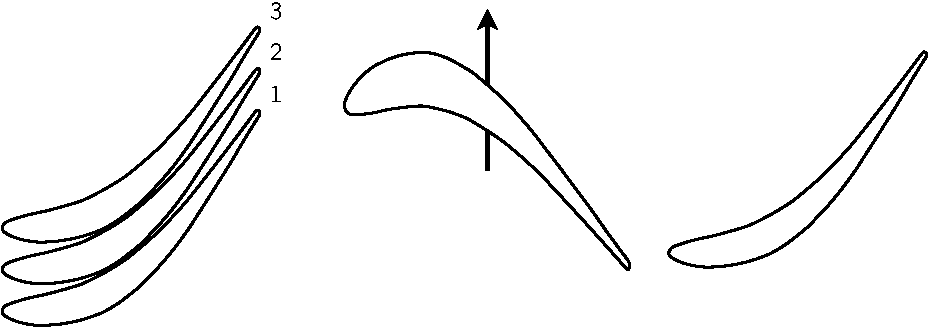
\includegraphics[width=.5\textwidth]{clocking_effect.pdf}
  \caption{Different clocking positions for a stator/rotor/stator
  configuration.}
  \label{fig:sm_nlh_clocking_effect}
\end{figure}
Fig.~\ref{fig:sm_nlh_clocking_effect} shows three
different clocking positions (sometimes also referred 
to as the indexing positions)
of the first stator
in a stator/rotor/stator configuration. In this figure,
the first clocking position is aligned with the second stator.
The second and the third clocking positions are not aligned with
the second stator, which may give different level of perceived
unsteadiness by the second stator. At a design phase, the engineer can choose any
relative position of the rows and thus any clocking position.
The relative position of both stator is of
prior interest to choose the best clocking position. 
In fact, the wakes that are shed behind the first stator
are cut by the rotor blades and transmitted to 
the second stator row. The stators being fixed, the wake of
the first stator is seen as a stationary wave in the second stator.
Hence, the importance of their relative position. For instance,
\citet{Huber1996} showed that
on their 1.5 stage turbine, the variation of efficiency due to clocking
position was equal to $0.8\%$ of efficiency points, showing the
importance of the clocking effect.

The brute force approach to compute the clocking effect on a
configuration is to consider all the relative positions. This means
that the geometry of the stator should be rotated for each new 
clocking position and hence a new unsteady computation should be 
run. The innovative procedure proposed by 
\citet{He2002} is to consider the clocking effect as a steady wave.
In fact, as both stator are fixed, a steady perturbation
shed behind the first stator is still steady in the second stator.
In terms of frequencies, a steady perturbation
can be assimilated to a zero frequency mode. 
In \citet{He2002} and \citet{Vilmin2009}, 
a perturbation with a zero frequency
is thus additionally computed. The clocking effect can then be evaluated by
post-processing the Fourier coefficient of the zeroth frequency mode.
Recently, the computation of clocking effects on
arbitrary configurations has been made possible
by \citet{Vilmin2013a}. This allows its use for 
pylon-rotor-rotor applications for instance, which
is the configuration encountered in an installed CROR.

\subsection{Numerical cost}
Compared to the LUR method, the number of equations to solve is 
not constant here. In fact, if $N$ denotes the number of harmonics
computed in total (sum of each harmonic of each perturbation)
and if $\mathdollar_{\text{RANS}}$ 
denotes the CPU and memory cost of
one steady computation, $2N$ harmonic equations and 
one time-average equation
are solved, thus
\begin{equation}
	\mathdollar_{\text{NLH}} = (2N+1) \times \mathdollar_{\text{RANS}}.
\end{equation}
However, \citet{Vilmin2006} do not apply the NLH formulation
to the turbulent equation (in their case, 
the one equation of \citet{Spalart1992}). Therefore,
as only five equations are solved using the NLH approach, the 
turbulent equation being solved as a steady one,
the cost becomes
\begin{equation}
	\mathdollar_{\text{NLH}} = \frac{5 \times (2N+1) + 1}{6} \times \mathdollar_{\text{RANS}}.
\end{equation}



\section{The \underline{N}on-\underline{L}inear 
\underline{F}requency \underline{D}omain method (NLFD)}
\label{sub:sm_nlfd}
%!TEX root = ../../../adrien_gomar_phd.tex

\subsection{Mono-frequential formulation}

Originally proposed by \citet{McMullen2001}, the NLFD
method relies on a simple observation: to develop Fourier-based methods, and in
particular the NLH method, one has made use of the Fourier
series to efficiently represent an unsteady signal.
This representation has then be used to develop the unsteady
equation into $2N+1$ steady equations: one time-averaged equation
and $2N$ perturbation equations, 
where $N$ denotes the number
of harmonic kept to compute the solution.
The problem is that the equations need to be 
resolved in the frequency domain meaning
that all the numerical techniques should be adapted: the numerical schemes,
the turbulent models and so on. The (smart) idea 
proposed by \citet{McMullen2001} is to
make use of the fast Fourier Transform and its inverse to
allow an easy implementation of the method into a classical time-domain code.
To explain the development of this method, let us first 
write Eq.~\eqref{eq:sm_nonlinear_convection_conservative} 
in a more general form:
\begin{equation}
	(\ref{eq:sm_nonlinear_convection_conservative})
	\Leftrightarrow
	\frac{\partial u}{\partial t} + R = 0,
	\label{eq:sm_nonlinear_convection_residual}
\end{equation}
with
\begin{equation}
	R = \frac{\partial}{\partial x} \left( 
	\frac{u^2}{2} \right).
\end{equation}
Let us now consider that both $u$ and $R$ are periodic
in time with respect to period $T = 2 \pi / \omega$
and can be written using a Fourier series:
\begin{equation}
	\begin{split}
		u(t) &= \sum_{k=-\infty}^{\infty} \widehat{u}_k e^{i k \omega t}, \\
		R(t) &= \sum_{k=-\infty}^{\infty} \widehat{R}_k e^{i k \omega t}.
	\end{split}
\end{equation}
Note that decomposing $R(t)$ into a Fourier series is equivalent
to use the Fourier decomposition of $u(t)$ and express
$R(t)$ using the Fourier coefficients $\widehat{u}_k$ of $u$
since the cross-terms that may arise are also expressed 
using the same complex exponentials. This comes from the fact
that multiplying a complex exponential with a complex exponential
just forms a new complex exponential at the power of the sum of the
two.
Injecting these decompositions into 
Eq.~\eqref{eq:sm_nonlinear_convection_residual} and taking into account
for the orthogonality of the complex exponentials:
\begin{equation}
	i k \omega \widehat{u}_k + \widehat{R}_k = 0, \: k \in [-\infty, \infty].
\end{equation}
As previously, only a small number of harmonics $N$ is kept and 
a pseudo-time ($\tau$) derivative is added to march the equations
in pseudo-time to the steady-state solutions of all the harmonics:
\begin{equation}
	\fbox{$
	\displaystyle \frac{\partial \widehat{u}_k}{\partial \tau} + 
	i k \omega \widehat{u}_k + \widehat{R}_k = 0, \: k \in [-N, N].
	$}
	\label{eq:sm_nlfd_subset_eq}
\end{equation}
The fact that $R(t)$ is expressed using its own Fourier series 
makes it simpler to implement 
as it avoids developing its expression using 
the complex coefficients $\widehat{u}_k$. 
However, $\widehat{R}_k$ must be evaluated. To do so, as depicted
in Fig.~\ref{fig:nlfd_principle}, \citet{McMullen2001}
propose to use an Inverse Fast-Fourier Transform (IFFT) to get
$u(t)$ from $\widehat{u}_k$. Then the considered governing equations
are used to evaluate $R(t)$ which leads to $\widehat{R}_k$
through a Fast-Fourier Transform (FFT). Finally, the next iteration value 
$\widehat{u}_k$
is evaluated by adding $\widehat{R}_k$ and 
the corresponding temporal derivative $i k \omega \widehat{u}_k$. All
harmonics are coupled through the IFFT and FFT operations
that needs all of the former to compute the counterpart temporal signal,
hence the coupling. Moreover, 
in the non-viscous Burger's equation framework, 
the term $u^\prime u^\prime$ is not neglected anymore compared to the
NLH approach and the computation of the deterministic stress is encompassed
by the FFT and IFFT operations.
\begin{figure}[htbp]
  \centering
  \includegraphics*[width=0.50\textwidth]{nlfd_principle.pdf}
  \caption{Simplified diagram of the computation of $\widehat{R}_k$ from $\widehat{u}_k$
  for the non-linear frequency domain method.}
  \label{fig:nlfd_principle}
\end{figure}

\subsection{Extensions}

\paragraph{Navier--Stokes equations}
The Navier--Stokes equations can be written in finite-volume,
semi-discrete form as:
\begin{equation}
	V \frac{\partial W}{\partial t} + R(W) = 0,
	\label{eq:navier_stokes_fv_sd}
\end{equation}
where $V$ is the volume of the cell and $W$
the vector of conservative variables.
This formulation is similar to
Eq.~\eqref{eq:sm_nonlinear_convection_residual} meaning that
nothing particular has to be made to derive this approach for
the Navier--Stokes equations. This is indeed attractive as the
method can be applied almost directly, except for the FFT and IFFT
step that should be added into the pseudo time loop.

\paragraph{Aeroelastic computations}
Since both the structural and the aerodynamic equations
are prone to time-periodic unsteadinesses,
\citet{Kachra2008} extended the NLFD approach to the strong coupling of
aeroelasticity within the two-dimensional Euler equations framework.
Both the fluid dynamics and the structural equations
are solved using the NLFD approach. They are coupled together 
every $15$ multigrid cycles.
A $2$D plunging and pitching airfoil is considered.
They demonstrate that with a one-harmonic NLFD computation the
flutter boundary of a NACA$64A010$ airfoil is correctly predicted.
This leads to a gain of one order of magnitude compared to a classical
time-marching procedure. 

\paragraph{Gradient-based method to determine the frequency}
\citet{McMullen2001} applied the NLFD to a cylinder
vortex shedding. This could be done as the frequency of the
vortex shedding was known \emph{a priori} from experimental
and numerical data. Note that this supposes that the
numerical and the experimental vortex shedding frequencies
are equal, which is generally not true~\cite{Kato1991}.
However, for a given cylinder, it is generally not
possible to know this frequency \emph{a priori}. This is why
\citet{McMullen2002, McMullen2006a}
proposed a gradient based method for determining the frequency
of a periodic phenomena where the frequency is unknown
\emph{a priori}. They argue that the frequency domain formulation
helps forming a gradient operator to find the period $T$ based
on the minimization of the residual of the unsteady equations.
They applied their algorithm to find the frequency of the vortex
shedding around a cylinder, and found it with a $3.5\%$ accuracy
compared to experimental data. Nevertheless, as a gradient method is 
used, a good initial guess is needed for the algorithm to
converge. This limits the methods to well-known unsteady
problems. Moreover, the prior interest of the NLFD method is
to reduce the cost compared to a classical time-marching scheme
to solve the unsteady periodic problem. One may ask
if applying the NLFD with an gradient based method is not finally
more costly than a classical time-marching scheme.

\paragraph{Optimum shape design}
\citet{Nadarajah2003} compared an optimum shape design 
strategy for pitching airfoils 
using both a classical time-marching scheme
and the NLFD scheme within the Euler equations
framework. It is shown that the NLFD method
gives the same accuracy for the gradient and the optimum with only 
three time-instants (namely $N=1$)
compared to $23$ time-instants needed for 
the time-marching approach.
\citet{Nadarajah2007} extended it
to the three-dimensional Navier--Stokes equations.
A wing undergoing a change 
in angle of attack as a function of time is computed and
it is demonstrated that
five instants (namely $N=2$) is sufficient to provide
accurate results.
\citet{Tatossian2011} applied it
to the aerodynamic shape optimization of hovering rotor blades
in the Euler framework.
The capability of 
their shape optimization process
to redesign the Caradonna–Tung experimental 
blade is assessed and gives a proof
of concept.

\paragraph{Adaptive method}
The problem of Fourier-based methods is that the higher
the number of harmonics computed, the higher the corresponding
CPU and memory cost. There is thus a need to optimize
the chosen number of harmonics.
\citet{Mosahebi2013} implemented an adaptive NLFD approach named
the p-NLFD. Based on the energy of the last mode compared
to the whole spectrum, the number of harmonics
is increased if a fixed threshold is not reached.
A speed-up of $2$ in terms of CPU cost and
memory reduction is observed for the case of a
vortex-shedding behind a cylinder.

\subsection{Cost of the method}
The NLFD method is close to the NLH approach in terms of number
of equations solved. However, at each time-step a fast Fourier transform
is performed to cast back the harmonics into the time-domain in order
to compute the residual $R(t)$. \citet{McMullen2006} argue
that the cost of the fast Fourier transform is less than the cost of 
the spatial derivatives. 
\citet{Kachra2008} quantitatively estimate it to be
approximately $2\%$ of the cost of one iteration, which is negligible.
Based on this affirmation, one can say that 
if $\mathdollar_{\text{RANS}}$ 
denotes the CPU and memory cost of
one steady computation, the cost of the NLFD method can be 
approximated by:
\begin{equation}
	\mathdollar_{\text{NLFD}} = (2N+1) \times \mathdollar_{\text{RANS}}.
\end{equation}
This evaluation of the cost is confirmed by numerical
simulations by \citet{McMullen2002}.

% ====================
% = HARMONIC BALANCE =
% ====================
\section{The \underline{H}armonic \underline{B}alance method (HB)}
\label{sec:sm_hb}
%!TEX root = ../../../adrien_gomar_phd.tex

The HB method has been originally
proposed by \citet{Hall2002}, at that time named
Harmonic Balance Technique (HBT).
It can be considered as an improvement of the NLFD
approach. In fact, instead
of using the fast Fourier transform to cast back the equations
to the time domain at each pseudo-iteration step, 
the equations are mathematically derived to be directly
computed into the time-domain.
To explain the method, we will again use the general form of 
the non-viscous Burger's equation as defined in
Eq.~\eqref{eq:sm_nonlinear_convection_residual}.
This thesis rely on the former work of \citet{ThesisSicot} who
implemented the harmonic balance method into the 
\textit{elsA}~\cite{Cambier2013} CFD code at CERFACS. 
Recently \citet{ThesisGuedeney} extended it to the
multi-frequential formulation, allowing contra-rotating
open rotor aeroelastic computations. This is why this
approach will be used in the current PhD work.

\subsection{Mono-frequential formulation}

Following the same approach as the non-linear frequency domain one,
it is considered that both $u$ and $R$ are periodic
in time with respect to period $T = 2 \pi / \omega$
and can be written using Fourier series:
\begin{equation}
	\begin{split}
		u(t) &= \sum_{k=-\infty}^{\infty} \widehat{u}_k e^{i k \omega t}, \\
		R(t) &= \sum_{k=-\infty}^{\infty} \widehat{R}_k e^{i k \omega t}.
		\label{eq:sm_hall_dft}
	\end{split}
\end{equation}
Injecting Eq.~\eqref{eq:sm_hall_dft} in 
Eq.~\eqref{eq:sm_nonlinear_convection_residual}, and considering
the orthogonality of the complex exponentials:
\begin{equation}
	i k \omega \widehat{u}_k + \widehat{R}_k = 0, \: k \in [-N, N].
	\label{eq:sm_hall_frequential_eq}
\end{equation}

In the same way as one uses Fourier coefficients to
evaluate the temporal signal,
one can reconstruct the Fourier coefficients using
temporal evaluations. These are taken at evenly spaced time instances
sampling the period $T = 2 \pi / \omega$. Moreover, 
according to the Nyquist-Shannon~\cite{Shannon1949} sampling theorem, 
at least $2N$ time instances are needed to capture $N$ frequencies. Actually
$2N+1$ time instances are used to prevent odd-even decoupling as
demonstrated by \citet{Weide2005}. $\widehat{u}_k$ can thus
be expressed in function of $u(t)$ using the inverse
Fourier transform:
\begin{equation}
	\widehat{u}_k = \frac{1}{2N+1} 
	\sum_{n=0}^{2N} u(t_n) e^{-i k \omega t_n}.
\end{equation}
If $E$ denotes the matrix composed of the elements 
$(E)_{k,n} = e^{-i (k - N) \omega t_n} / 2N+1$, one can write $\widehat{u}_k$
and $\widehat{R}_k$ as:
\begin{equation}
	\begin{split}
		\widehat{u}_k &= E u^\star, \\
		\widehat{R}_k &= E R^\star,
	\end{split}
	\label{eq:sm_matrix_fourier_operator}
\end{equation}
where $u^\star$ and $R^\star$ 
denote the vectors formed of all the evaluations of $u$
and $R$, respectively,
made at $2N+1$ time instances uniformly sampling the period of interest:
\begin{equation}
	\begin{split}
		u^\star &= [u(t_0) \cdots u(t_{2N})], \\
		R^\star &= [R(t_0) \cdots R(t_{2N})].
	\end{split}
\end{equation}
$E$ can thus be named the Fourier matrix.
Note that conversely, using the inverse Fourier matrix $E^{-1}$:
\begin{equation}
	\begin{split}
		u^\star &= E^{-1} \widehat{u}_k \\
		R^\star &= E^{-1} \widehat{R}_k.
	\end{split}
	\label{eq:sm_sampling_hb_var}
\end{equation}
Injecting the matrix formulation of 
Eq.~\eqref{eq:sm_matrix_fourier_operator} in 
Eq.~\eqref{eq:sm_hall_frequential_eq}
gives:
\begin{equation}
	i \omega K E u^\star + E R^\star = 0,
\end{equation}
where $K$ is a diagonal matrix formed of all the $k \in [-N, N]$.
Note that first, the matrix formulation encompass all harmonics
$k \in [-N, N]$ and second, it does not require the
orthogonality of the complex exponentials.
Now multiplying the equation by the inverse Fourier matrix $E^{-1}$:
\begin{equation}
	i \omega E^{-1} K E u^\star + R^\star = 0,
	\label{eq:sm_hb_matrix_form_mono}
\end{equation}
where $R^\star$ can now be substituted:
\begin{equation}
		i \omega E^{-1} K E u^\star + 
		\displaystyle \frac{\partial}{\partial x}
		\frac{(u^\star)^2}{2} = 0.
\end{equation}
What happened here is that instead of developing $R(t)$
in the frequency domain as made with the NLH approach,
which is tedious, this term is kept
in this form through all the development process. 
Since $R(t)$ only includes spatial derivatives, no temporal non-linear
terms
arise by using the Fourier decomposition. Thus, multiplying it
by the inverse Fourier matrix leads to the unity matrix. 
$R(t)$ is then simply evaluated at $2N+1$ time instances.

This approach is really close to the NLFD method.
The higher order perturbation terms are taken into account
in the equations.
% The reader might observe that we are introducing the discrete Fourier
% transform and its inverse. This is close to the fast Fourier transform
% and its inverse, as proposed by \citet{McMullen2001}. 
However,
as the development is on the equations and not during the time loop,
we get $2N+1$ steady equations, by definition in the time
domain, that are coupled by a source term.
The source term appears as a spectral operator defined as:
\begin{equation}
	D_t = i \omega E^{-1} K E.
	\label{eq:sm_hb_mono_source_term_matrix}
\end{equation}

To compute $D_t$, \citet{Hall2002}
inverse the Fourier matrix $E$.
In an easier way, \citet{Gopinath2005} provided 
an analytical formulation of the source term defined 
in Eq.~\eqref{eq:sm_hb_mono_source_term_matrix} and 
named the HB approach the Time Spectral Method (TSM).
It is a matrix operator whose elements are defined as:
\begin{equation}
  (D_t)_{k, n} =
  \begin{cases}
    \frac{\pi}{T}(-1)^{k-n}\csc\left(\frac{\pi
        (k-n)}{2N+1}\right) &, \, k\neq n,\\
    0 &, \, k=n.
  \end{cases}
  \label{eq:sm_hb_mono_source_term_analytic}
\end{equation}
The main difference with the NLFD approach
is that the source term matrix $D_t$ is known at the first iteration and does
not change, meaning that we do not spend time computing a
fast Fourier transform and its inverse at each time-step.
Finally, adding a pseudo-time ($\tau$) derivative to 
time march the equations to the steady state, 
the mono-frequential formulation of 
Eq.~\eqref{eq:sm_nonlinear_convection_conservative} in the harmonic
balance framework is given by:
\begin{equation}
	\fbox{$
	\displaystyle \frac{\partial u^\star}{\partial \tau} + 
	D_t (u^\star) + 
	\displaystyle \frac{\partial}{\partial x}
		\frac{(u^\star)^2}{2} = 0
	$}
\end{equation}
with $D_t$ defined using Eq.~\eqref{eq:sm_hb_mono_source_term_analytic}.
As for the NLFD method, the term $u^\prime u^\prime$
is not neglected in the current approach.

\subsection{Multi-frequential formulation}
\label{sec:sm_hb_multi}
In the
framework of almost-periodic functions~\cite{Besicovitch1932},
such a function $f(t)$ (which is composed of multiple
frequencies non necessarily harmonically related) can be approximated
by an almost-periodic
discrete Fourier transform:
\begin{equation}
	f(t) \approx \sum_{k=-N}^{N} \widehat{f}_k 
	e^{i \omega_k t}.
\end{equation}
In this framework, \citet{Gopinath2007} and \citet{Ekici2007} 
extended the harmonic balance approach to
a multi-frequential formulation. To do so, they considered
a Fourier matrix defined as:
\begin{equation}
	(E)_{k,n} = \frac{1}{2N+1} e^{-i \omega_{k-N} t_n},
\end{equation}
where $N$ is the chosen number of frequencies.
Note that replacing $\omega_{k-N}$ by $(k - N) \omega$ gives
the mono-frequential inverse Fourier matrix back. 
However, in the multi-frequential case, the inverse Fourier matrix
$E^{-1}$ has to be numerically computed from $E$. Actually, as demonstrated by 
\citet{Gopinath2007}, it is easier to express $E^{-1}$ analytically,
compute its temporal derivative (that is hence analytical too) 
and inverse it numerically to obtain $E$. In fact, the source term
can be written as $D_t = \frac{\partial E^{-1}}{\partial t} E$
which ease its computation.

Using the same process as for the mono-frequential formulation,
Eq.~\eqref{eq:sm_nonlinear_convection_residual} becomes:
\begin{equation}
	i E^{-1} P E u^\star + R^\star = 0,
\end{equation}
where $P$ is a diagonal matrix formed of all the angular frequencies $\omega_k$.
Note that the exponentials do not need to form an
orthogonal family here. The only need is to have the multi-frequential
Fourier matrix $E$ to be invertible which is the case~\cite{Ekici2007}.
This is really close to the mono-frequential formulation given
in Eq.~\eqref{eq:sm_hb_matrix_form_mono}.
Finally, adding a pseudo-time ($\tau$) derivative 
to time-march the equations to the steady state,
the multi-frequential formulation of 
Eq.~\eqref{eq:sm_nonlinear_convection_conservative} in the harmonic
balance framework reads:
\begin{equation}
	\fbox{$
	\displaystyle \frac{\partial u^\star}{\partial \tau} +
	D_t (u^\star) + 
	\displaystyle \frac{\partial}{\partial x}
		\frac{(u^\star)^2}{2} = 0
	$}
\end{equation}
with $D_t$ defined as:
\begin{equation}
	D_t = i E^{-1} P E,
	\label{eq:sm_multi_spectral_operator}
\end{equation}
and again $u^\star = [u(t_0) \cdots u(t_{2N})]$ 
and $R^\star = [R(t_0) \cdots R(t_{2N})]$.

\subsection{Extensions}

\paragraph{Navier--Stokes equations}
As for the NLFD approach, since the 
Navier--Stokes equations can be written in finite-volume,
semi-discrete form as:
\begin{equation}
	V \frac{\partial W}{\partial t} + R(W) = 0,
\end{equation}
nothing particular has to be made to derive this approach for
the Navier--Stokes equations, except adding the source term computation
in the time-loop.
This shows its advantage over the NLFD and particularly over the NLH method.

\paragraph{Turbomachinery computations}
Originally, the HB method has been developed for 
turbomachinery applications.
\citet{Hall2002} applied the method to the computation
of the flutter boundary of the front stage rotor 
of a modern high-pressure transonic compressor. To reduce the
computational domain to a single blade passage, 
a phase-lagged boundary condition is used at the azimuthal
interfaces:
\begin{equation}
	\widehat{u}_{k, U} = \widehat{u}_{k, L} e^{i \sigma k},
\end{equation}
for $k \in [-N, N]$, where subscript $U$ and $L$ denote
respectively the upper and lower azimuthal boundaries, and
$\sigma$ denotes the inter-blade phase angle. This boundary
condition allows to compute isolated aeroelastic configurations
using only one blade-passage.
\Citet{Weide2005} extended the approach to take into account
for the periodic boundary conditions when the equations are solved in the
cartesian coordinate system. The efficiency of the
method was demonstrated with the NASA-Stage~$35$ compressor. In that case,
engineering accuracy is obtained with only $N=5$ harmonics.
Nothing is said on the strategy used at the rows interface.

\citet{Ekici2007} and \citet{Gopinath2007}
extended the method to a multi-frequential formulation. 
As such, it can then be applied to multi-stage
configurations. Both of them demonstrated the application of
the method on
a two-dimensional multi-stage compressor called
configuration~D. 
The strategy used by \citet{Ekici2007} 
to exchange the variables at
the rows interface is schematically represented 
in Fig.~\ref{fig:bnd_sliding_ekici2007}.
\begin{figure}[htp]
  \centering
  \includegraphics*[scale=0.25]{bnd_sliding_ekici2007.pdf}
  \caption{Exchange of the variable at rows interface as described by \citet{Ekici2007}.}
  \label{fig:bnd_sliding_ekici2007}
\end{figure}
The temporal and azimuthal variations 
of the field (here represented as $u (\theta_i, t_i)$)
in row $i$ are Fourier transformed first with
respect to time, and then
to space to obtain the spatio-temporal modes $\widetilde{u}_i$.
At the interface, these modes are transmitted using a non-reflecting
boundary condition filtering the spurious modes. In fact, as only some
temporal modes are computed using the HB approach, only
those will be kept when transmitted to the opposite row.
Finally, the inverse operations are carried out in
the opposite row: first an inverse
azimuthal Fourier transform is performed and second an inverse
temporal Fourier transform is done which gives $u (\theta_j, t_j)$
in row $j$.
\citet{Gopinath2007} used a different approach to transfer
the information at the interface as shown
in Fig.~\ref{fig:bnd_sliding_gopinath2007}. 
\begin{figure}[htp]
  \centering
  \includegraphics*[scale=0.25]{bnd_sliding_gopinath2007.pdf}
  \caption{Exchange of the variable at rows interface as described by \citet{Gopinath2007}.}
  \label{fig:bnd_sliding_gopinath2007}
\end{figure}
In most time-domain solver,
a sliding mesh treatment exists to interpolate azimuthal variations
between consecutive rows. Therefore, \citet{Gopinath2007}
interpolates temporally the field on the time instances used for
the HB computation in
the opposite row. To do so, they used a temporal Fourier
transform combined with an inversed one using the time samples
of the opposite row.
Then, they applied the sliding mesh treatment
to spatially transfer the information. Again, as spurious effects
can appear, the time interpolation is done, not on the $2N+1$ samples
of the opposite row, but rather on $2 \times (2N+1)$ samples. This over-sampling
helps isolating the spurious effects on the higher harmonics to suppress them.


\citet{Ekici2008a} applied the multi-frequential method
to the effect of wake passing on the vibration of
a turbine blade. Note that the stator is modeled
by an unsteady wake injection but not computed.
Two frequencies are involved: the blade passing
frequency of the opposite row, here the
stator row that is modeled through an unsteady wake injection,
and the aeroelastic frequency, justifying the use
of the multi-frequential formulation.


At CERFACS, \citet{JSicot2012} implemented the harmonic balance 
into the \textit{elsA}~\cite{Cambier2013} CFD code
and analyzed the rotor-stator interaction in a subsonic
compressor. To reduce the computational domain, 
phase-lag boundary conditions are implemented
using the general expression of the phase-lag due to
different number of blades in the different rows 
provided by \citet{Gerolymos1991}:
\begin{equation}
 	\sigma = - 2 \pi \sign \left(\Omega_{cur} - \Omega_{opp} \right) 
 	\left(1 - \frac{B_{opp}}{B_{cur}}\right),
\end{equation} 
where $\Omega$ denotes the rotation speed, $B$ the number
of blade and subscript $opp$ and $cur$, respectively, the
opposite and the current row. The same treatment as \citet{Gopinath2007}
is used at the interface.
\citet{ThesisGuedeney} extended this to the multi-frequential framework.
He showed that unsteadinesses coming from upstream and downstream
rows can be retrieve with a good accuracy using only a limited 
number of harmonics.

\paragraph{Choice of the frequencies for the multi-frequential formulation}
\label{par:choice_of_frequencies}

Due to the non-linearity of the considered
equations, the presence 
of two or more base frequencies can lead to
the emergence of combinations of them.
This leads to a set of possible frequencies that 
is two-dimensional or more. As an infinite number of frequencies
can not be computed, this set 
has to be truncated. In the electronic literature,
\citet{Kundert1988} propose two types of truncation:
the "square grid" and the "diamond grid" truncations.
These are schematically represented in Fig.~\ref{fig:dream_hb_truncation}.
Dots represent frequencies that are computed by the multi-frequential
harmonic balance approach.
\begin{figure}[htp]
  \centering
  \subfigure[square grid]{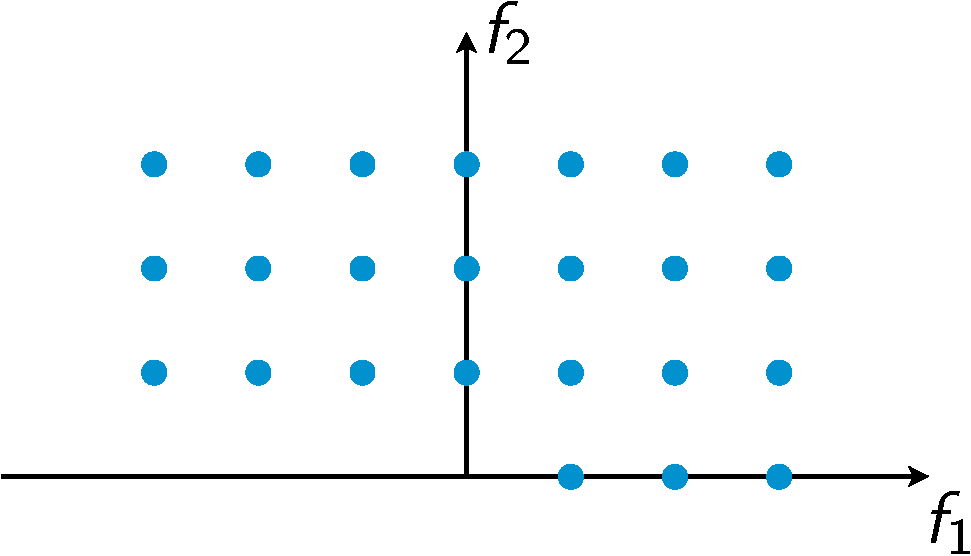
\includegraphics[width=.25\textwidth]{truncation_square.pdf}}
  \subfigure[diamond grid]{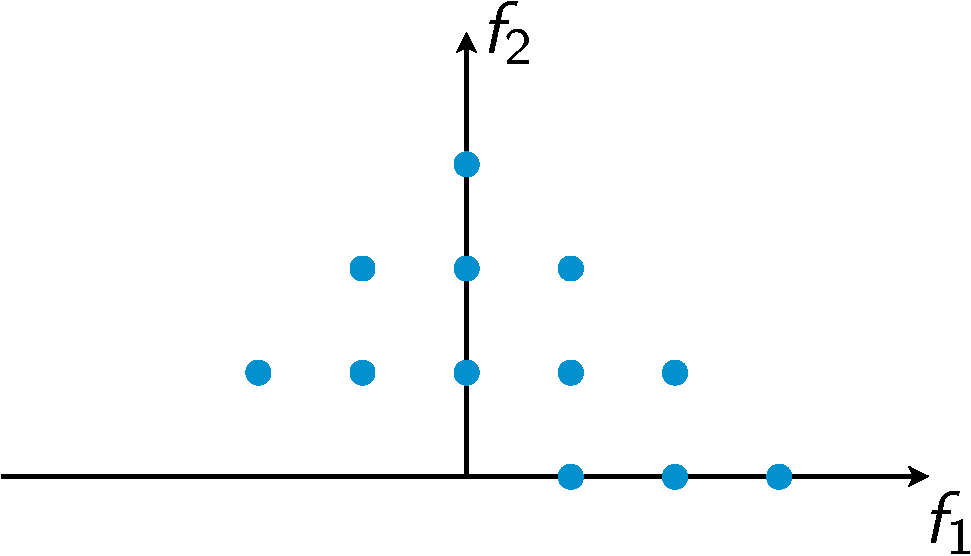
\includegraphics[width=.25\textwidth]{truncation_diamond.pdf}}
  \subfigure[cross grid]{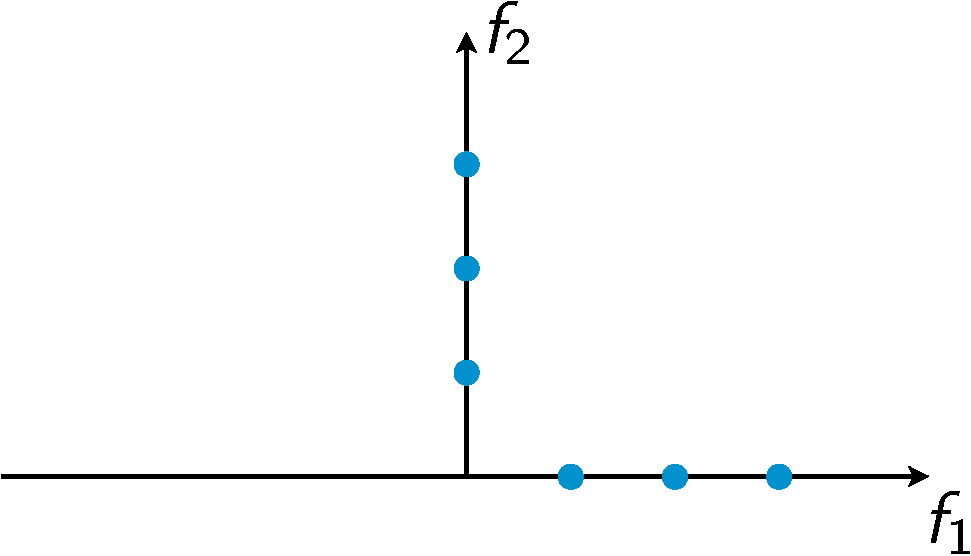
\includegraphics[width=.25\textwidth]{truncation_cross.pdf}}
  \caption{Truncation grids for reducing the set of frequencies of multi-frequential
  harmonic balance computations.}
  \label{fig:dream_hb_truncation}
\end{figure}
In the turbomachinery literature, \citet{Gopinath2007} follows the
diamond grid pattern while \citet{Ekici2007} seems to choose a
square grid pattern. In his PhD thesis, \citet{ThesisGuedeney}
first choose the frequencies by knowing which one emerge based on
a reference classical time-marching computation. Of course,
this approach can only be done \emph{a posteriori} which limits
the predictability of the method. He
also made computations with a "cross grid" truncation 
(shown in Fig.~\ref{fig:dream_hb_truncation}), this new type 
of truncation scheme only considers the harmonics of the
base frequencies. \citet{ThesisGuedeney} showed that this
truncation pattern gives
similar if not better results that the
"diamond grid" truncation pattern.  This "cross grid"
truncation pattern will be used in the current PhD work
when using the multi-frequential approach.

\paragraph{Aeroelastic simulations}

\citet{Thomas2002a} used the method to
determine the Limit-Cycle Oscillation (LCO) solution
of a transonic airfoil configuration using the
Euler equations and \citet{Thomas2004b} extended
it to the viscous Navier-Stokes equations.
For external-flow aeroelasticity, the HB approach has 
been thoroughly 
validated by \citet{Gopinath2005, JSicot2008, Woodgate2009, JDufour2009}, 
mostly for the AGARD test cases of \citet{Davis1982}. 
\citet{JDufour2009} highlight the benefits of using a 
non-linear approach for oscillating-flap simulations
compared to linearized approaches. A one-harmonic HB simulation
gives results comparable to an expensive time-marching simulation.
\citet{Huang2013} applied the mono-frequential
HB method to the flutter prediction of the 
$11\textsuperscript{th}$ 
standard configuration for aeroelasticity~\cite{Fransson1999}.
They show that with only one harmonic, the local
harmonic response of the fluid is superimposed
with the results of a time-marching simulation.
The same study has been performed in this PhD work
as detailed in Chap.~\ref{cha:stcf11}
and the same conclusions are drawn. These results have been
published as \citet{JSicot2012}.
In the context of the current thesis,
\citet{JSicot2013} applied the multi-frequential method to the
aeroelasticity of a contra-rotating fan, proving
the maturity of the method.


\paragraph{Transient problems}
\citet{Mavriplis2012} extended the method to 
an hybrid polynomial-harmonic balance approaches. 
It allows to use the method for maneuver simulations, 
where a part of the simulation exhibits a physical transient.
The method is also extended to overlapping mesh grids.

% \paragraph{Time sampling in the case of multi-frequential formulation}
% \citet{Gopinath2007} and \citet{Ekici2007}
% applied the multi-frequential method to
% a two-dimensional multistage compressor called
% configuration D. \citet{Ekici2007} use
% $3N+1$ evenly spaced 
% time instances to improve the condition number
% of the source term while \citet{Gopinath2007}
% stays with $2N+1$ evenly spaced time instances.
% \citet{Ekici2008a} applied the multi-frequential method
% to the effect of wake passing on the vibration of
% a turbine blade and uses $2N+1$ evenly spaced
% time instances are considered.
% \citet{JGuedeney2013} introduce non-uniform 
% time instances to minimize the condition number of multi-frequential
% computations. 
% The effect of the condition number on the stability
% of the computations is assessed along with algorithms
% to optimize the choice of the time instances.
% This allows to drastically reduce the condition number for
% any combination of frequencies, 
% while keeping only $2N+1$ samples.
% The method is then applied
% to a $1.5$ stage subsonic compressor.
% Note that a part of this work has been done in this
% thesis and will be detailed latter on.

\paragraph{Gradient-based method to determine the frequency}
With the same approach as \citet{McMullen2002}, \citet{Gopinath2006}
developed a gradient-based method to estimate the frequency of a 
vortex shedding behind a cylinder and a NACA0012 airfoil 
at high angle of attack using the harmonic balance approach.
The results are superimposed with a classical time-marching approach ones.

\paragraph{Optimum shape design}
\citet{Thomas2005b} used an automatic 
differentiation compiler to derive an adjoint code
from their harmonic balance code. This adjoint code is then
evaluated on the NLR~7301 supercritical airfoil section.
The computation of the sensibilities is finally
classically compared to a finite-difference and shows
to be in good agreement with these, validating
the given approach.

\paragraph{Adaptive method}
\citet{Maple2004} presented an adaptive harmonic
balance approach. The number of harmonics is increased
if the energy of the last harmonic divided by the cumulative
sum of the energy of each harmonic is larger than a 
given threshold. During the first iterations, only
a low number of harmonic is kept. Then, when the flow
is almost converged, the adaptive harmonic balance
approach is used. This ensures that higher order harmonics
are not injected at the first iterations, when the
flow is not physical. A $86\%$ reduction in time (and
in memory footprint) is seen compared to a resolved (converged in
terms of harmonics $N$) harmonic
balance computation. This has to be compared to
the $2$ factor speed-up observed by \citet{Mosahebi2013}
with an adaptive NLFD approach.

\subsection{Cost of the method}
\label{sec:sm_hb_cost}
As mentioned before, the cost of the method is linked to
the number of simulated time instances.
In fact, each new time instance corresponds to an additional steady computation.
Thus, if \mbox{$2N+1$} time instances are considered and if $\mathdollar_{\text{RANS}}$ 
denotes the CPU and memory cost of
one steady computation, the cost of the HB method can be 
approximated by:
\begin{equation}
	\mathdollar_{\text{HB}} = (2N+1) \times \mathdollar_{\text{RANS}}.
\end{equation}
Note that \citet{Ekici2007,Ekici2008a} use $3N+1$
time instances or more to solve the bad conditioning of the
source term when using the multi-frequential formulation. 
'This will be detailed latter on this thesis in 
Chapter~\ref{cha:limitations_condition_number} and an innovative solution
will be proposed. In that
case, the cost is bigger and scales with the chosen number
of time instances.


% ===================================
% = Periodic flows in turbomachines =
% ===================================
\section{Periodic flows in turbomachines}
\label{sec:sm_hudson}
%!TEX root = ../../../adrien_gomar_phd.tex

In this thesis, the final application is contra-rotating open rotor
configurations. To bound Fourier-based time methods for such
applications, we propose a classification of the
unsteady phenomena that can be computed using such approaches.

Inspired by \citet{Hodson1998},
a diagram presenting the unsteadinesses seen in 
a CROR is shown in Figure~\ref{fig:hudson}. A distinction
is made between unsteadinesses whose frequencies are
known or not.
\begin{figure}[htp]
  \centering
  \includegraphics*[scale=0.8]{hudson.pdf}
  \caption{Main unsteady phenomenon seen by contra-rotating
  open rotors. Bold blue text highlights applications that can
  be treated with the harmonic balance implementation available for the
  current thesis and underlined red text shows additional applications
  made possible by extensions available in the literature.}
  \label{fig:hudson}
\end{figure}
From the bibliography presented previously, almost all
unsteady flows can be computed using Fourier-based time methods.
The current implementation of the HB method available for
this thesis is able to compute all the unsteadinesses highlighted
by a bold text. In the literature, the presented work of 
\citet{Mavriplis2012} allows to compute transient unsteady flow
resulting from a change of operating point and/or a maneuver and
the work of \citet{McMullen2002} and \citet{Gopinath2006} allows
to capture periodic flows whose frequency is unknown. These two
kinds of unsteadiness are added
to the current panel of applications that can
be treated by Fourier-based time methods. Let us note
that the gradient algorithm presented by \citet{McMullen2002}
and \citet{Gopinath2006} is only able to converge when a 
good approximate of the solution is given, meaning
that this strategy fails when one has no estimate
of the value of the frequency for the considered phenomenon.
It can also be inferred that using such an optimization algorithm
coupled with a Fourier-based time method
might require more computational time than a classical time-marching scheme,
which limits its applicability to academical configurations.



\chconclu{Four Fourier-based methods have been presented in this chapter.
The main mathematical development have been demonstrated and 
the hypothesis/weakness of each method has been highlighted.
In particular, the presented harmonic balance method can
treat both mono and multi-frequential applications. One
unsteady equation is transformed into a subset of $2N+1$
steady-state equations coupled by a source term. This last
is analytical in the mono-frequential formulation and
of matrix form in the multi-frequential framework.
The large literature available on these methods shows that
they are ready for industrial, numerically hard
unsteady applications. Moreover, the method is able to
efficiently compute aeroelastic phenomenon on 
contra-rotating configurations explaining its
use in the present thesis.}
